\begin{pages}
    \begin{Rightside}
    \selectlanguage{greek}
        \beginnumbering
        \pstart[
        			\chapter{Ὁ τοῦ θηρίου ἀριθμός}
        			\markboth{The Number of the Beast}
				]
		\renewcommand{\LettrineFontHook}{\PHtitl}
		\lettrine[lines=3]{Κ}{αὶ} εἶδον ἐκ τῆς θαλάσσης θηρίον ἀναβαῖνον, ἔχον κέρατα δέκα καὶ κεφαλὰς ἑπτά, καὶ ἐπὶ τῶν κεράτων αὐτοῦ δέκα διαδήματα, καὶ ἐπὶ τὰς κεφαλὰς αὐτοῦ ὀνόματα βλασφημίας. καὶ τὸ θηρίον ὃ εἶδον ἦν ὅμοιον παρδάλει, καὶ οἱ πόδες αὐτοῦ ὡς ἄρκου, καὶ τὸ στόμα αὐτοῦ ὡς στόμα λέοντος. καὶ ἔδωκεν αὐτῷ ὁ δράκων τὴν δύναμιν αὐτοῦ καὶ τὸν θρόνον αὐτοῦ καὶ ἐξουσίαν μεγάλην. 
		\pend
		\pstart
		καὶ μίαν ἐκ τῶν κεφαλῶν αὐτοῦ ὡς ἐσφαγμένην εἰς θάνατον, καὶ ἡ πληγὴ τοῦ θανάτου αὐτοῦ ἐθεραπεύθη. καὶ ἐθαυμάσθη ὅλη ἡ γῆ ὀπίσω τοῦ θηρίου, καὶ προσεκύνησαν τῷ δράκοντι ὅτι ἔδωκεν τὴν ἐξουσίαν τῷ θηρίῳ, καὶ προσεκύνησαν τῷ θηρίῳ λέγοντες Τίς ὅμοιος τῷ θηρίῳ, καὶ τίς δύναται πολεμῆσαι μετ’ αὐτοῦ; 
		\pend
		\pstart
		καὶ ἐδόθη αὐτῷ στόμα λαλοῦν μεγάλα καὶ βλασφημίας, καὶ ἐδόθη αὐτῷ ἐξουσία ποιῆσαι μῆνας τεσσεράκοντα δύο. καὶ ἤνοιξεν τὸ στόμα αὐτοῦ εἰς βλασφημίας πρὸς τὸν Θεόν, βλασφημῆσαι τὸ ὄνομα αὐτοῦ καὶ τὴν σκηνὴν αὐτοῦ, τοὺς ἐν τῷ οὐρανῷ σκηνοῦντας. 
		\pend
		\pstart
		καὶ ἐδόθη αὐτῷ ποιῆσαι πόλεμον μετὰ τῶν ἁγίων καὶ νικῆσαι αὐτούς, καὶ ἐδόθη αὐτῷ ἐξουσία ἐπὶ πᾶσαν φυλὴν καὶ λαὸν καὶ γλῶσσαν καὶ ἔθνος. καὶ προσκυνήσουσιν αὐτὸν πάντες οἱ κατοικοῦντες ἐπὶ τῆς γῆς, οὗ οὐ γέγραπται τὸ ὄνομα αὐτοῦ ἐν τῷ βιβλίῳ τῆς ζωῆς τοῦ Ἀρνίου τοῦ ἐσφαγμένου ἀπὸ καταβολῆς κόσμου. Εἴ τις ἔχει οὖς, ἀκουσάτω. εἴ τις εἰς αἰχμαλωσίαν, εἰς αἰχμαλωσίαν ὑπάγει· εἴ τις ἐν μαχαίρῃ ἀποκτενεῖ, δεῖ αὐτὸν ἐν μαχαίρῃ ἀποκτανθῆναι. Ὧδέ ἐστιν ἡ ὑπομονὴ καὶ ἡ πίστις τῶν ἁγίων. 
		\pend
		\pstart
		Καὶ εἶδον ἄλλο θηρίον ἀναβαῖνον ἐκ τῆς γῆς, καὶ εἶχεν κέρατα δύο ὅμοια ἀρνίῳ, καὶ ἐλάλει ὡς δράκων. καὶ τὴν ἐξουσίαν τοῦ πρώτου θηρίου πᾶσαν ποιεῖ ἐνώπιον αὐτοῦ. καὶ ποιεῖ τὴν γῆν καὶ τοὺς ἐν αὐτῇ κατοικοῦντας ἵνα προσκυνήσουσιν τὸ θηρίον τὸ πρῶτον, οὗ ἐθεραπεύθη ἡ πληγὴ τοῦ θανάτου αὐτοῦ. καὶ ποιεῖ σημεῖα μεγάλα, ἵνα καὶ πῦρ ποιῇ ἐκ τοῦ οὐρανοῦ καταβαίνειν εἰς τὴν γῆν ἐνώπιον τῶν ἀνθρώπων. 
		\pend
		\pstart
		καὶ πλανᾷ τοὺς κατοικοῦντας ἐπὶ τῆς γῆς διὰ τὰ σημεῖα ἃ ἐδόθη αὐτῷ ποιῆσαι ἐνώπιον τοῦ θηρίου, λέγων τοῖς κατοικοῦσιν ἐπὶ τῆς γῆς ποιῆσαι εἰκόνα τῷ θηρίῳ, ὃς ἔχει τὴν πληγὴν τῆς μαχαίρης καὶ ἔζησεν. καὶ ἐδόθη αὐτῷ δοῦναι πνεῦμα τῇ εἰκόνι τοῦ θηρίου, ἵνα καὶ λαλήσῃ ἡ εἰκὼν τοῦ θηρίου, καὶ ποιήσῃ ἵνα ὅσοι ἐὰν μὴ προσκυνήσωσιν τῇ εἰκόνι τοῦ θηρίου ἀποκτανθῶσιν. 
		\pend
		\pstart
		καὶ ποιεῖ πάντας, τοὺς μικροὺς καὶ τοὺς μεγάλους, καὶ τοὺς πλουσίους καὶ τοὺς πτωχούς, καὶ τοὺς ἐλευθέρους καὶ τοὺς δούλους, ἵνα δῶσιν αὐτοῖς χάραγμα ἐπὶ τῆς χειρὸς αὐτῶν τῆς δεξιᾶς ἢ ἐπὶ τὸ μέτωπον αὐτῶν, καὶ ἵνα μή τις δύνηται ἀγοράσαι ἢ πωλῆσαι εἰ μὴ ὁ ἔχων τὸ χάραγμα τὸ ὄνομα τοῦ θηρίου ἢ τὸν ἀριθμὸν τοῦ ὀνόματος αὐτοῦ. Ὧδε ἡ σοφία ἐστίν. ὁ ἔχων νοῦν ψηφισάτω τὸν ἀριθμὸν τοῦ θηρίου· ἀριθμὸς γὰρ ἀνθρώπου ἐστίν. καὶ ὁ ἀριθμὸς αὐτοῦ ἑξακόσιοι ἑξήκοντα ἕξ.
		\pend
        \endnumbering
    \end{Rightside}
    \begin{Leftside}
        \beginnumbering
        \pstart[
        			\chapter{The Number of the Beast}
				]		
		\renewcommand{\LettrineFontHook}{\Zallmanfamily}
		\lettrine[lines=3]{A}{nd} I saw coming out of the sea a beast (monster) having ten horns and seven heads and upon its horns (there were) ten crowns; and upon its heads (were the names) of blasphemy. And the beast which I saw was like a leopard and its feet (were) like (those) of a bear and its mouth (was) like the mouth of a lion. And the dragon gave the beast his power and his throne and his great authority. 
		\pend
		\pstart
		And one of its heads was (as if it was) wounded into death (i. e. it had a fatal wound) but (and) its fatal wound was healed. And all the Earth was astonished at (wondered after) the great beast and they worshipped the dragon, for it gave (his) power to the beast; and they worshipped the beast saying, “Who is like the beast and who is able to fight (with) it?” 
		\pend
		\pstart
		And there was given to it a mouth to speak great (things) and (to speak) blasphemies; and there was (also) given to it (the authority) to do (the above mentioned things) for forty-two months. And it opened its mouth to (speak) blasphemous(ly) to God (in order) to blaspheme (not only) (against) His name (but also against) His tabernacle (tent) and those dwelling in Heaven. 
		\pend
		\pstart
		And there was given to it (the authority) to make war with the holy (men, people) and (the authority) to prevail over them; and it was given the authority over every tribe and country and tongue (language) and peoples. And all the inhabitants upon the Earth worshipped it, (the ones) whose names are not written in the book of life of the slain Lamb from the foundation of the cosmos (universe, Earth). If (some)one has an ear, let him hear! If one (is destined to go) into captivity, into captivity he goes; if one kills (someone else) by sword, he will (himself) need to be killed by sword; thus (here) is the patient endurance and the faith of the holy. 
		\pend
		\pstart
		And I saw another beast (monster) ascending from (out of?) the Earth and it had two horns (like those of) a lamb and it speaks like (the, a) dragon. And it exercises the entire authority of the first beast before (in front of) it; and it makes the Earth and those dwelling therein worship the first beast — (namely the one) whose fatal wound was healed. And it makes (creates) great signs, so that even fire is made to descend from Heaven into the Earth before the people (of the Earth). 
		\pend
		\pstart	
		And it deceives the inhabitants of the Earth through (the usage of) signs which were given to it to perform (do) them before the beast; (and it was) saying to the inhabitants of the Earth (and ordered them) to create idols to the beast which has the fatal sword wound and lived. And there was given to it (the authority) to give a soul (life) to the idol of the beast so that even the idol of the beast might (be able to) speak; and it made (it) so that, whoever does not worship the idol of the beast, dies. 
		\pend
		\pstart
		And it made (forced) everyone — the small and the large; the rich and the poor; and the free and the slaves — to give them(selves) a mark upon their right hand or upon their forehead, so that one may neither buy nor sell (wares) unless he has the mark of the name of the beast or (the mark) of the number of its names. Thus (here) is the wisdom. Let him who has a mind calculate the number of the beast; for the number is (the number) of humans; and its number is six-hundred sixty-six. 
		\pend
        \endnumbering
    \end{Leftside}

\end{pages} 
\Pages

\clearpage
\thispagestyle{empty}
\null\vfill
\settowidth\longest{\huge\itshape […] and when I turned around I saw}
\begin{center}
\parbox{\longest}{%
  \raggedright{\huge\itshape%
    ``And I saw coming out of the sea a beast having ten horns and seven heads and upon its horns (there were) ten crowns.'' \par\bigskip
  }
  \raggedleft\Large\MakeUppercase{``The Number of the Beast is 666'' — William Blake, 1805}\par%
}
\vfill\vfill
\clearpage\newpage
\end{center}
\newpage
\thispagestyle{empty}
\begin{center}
	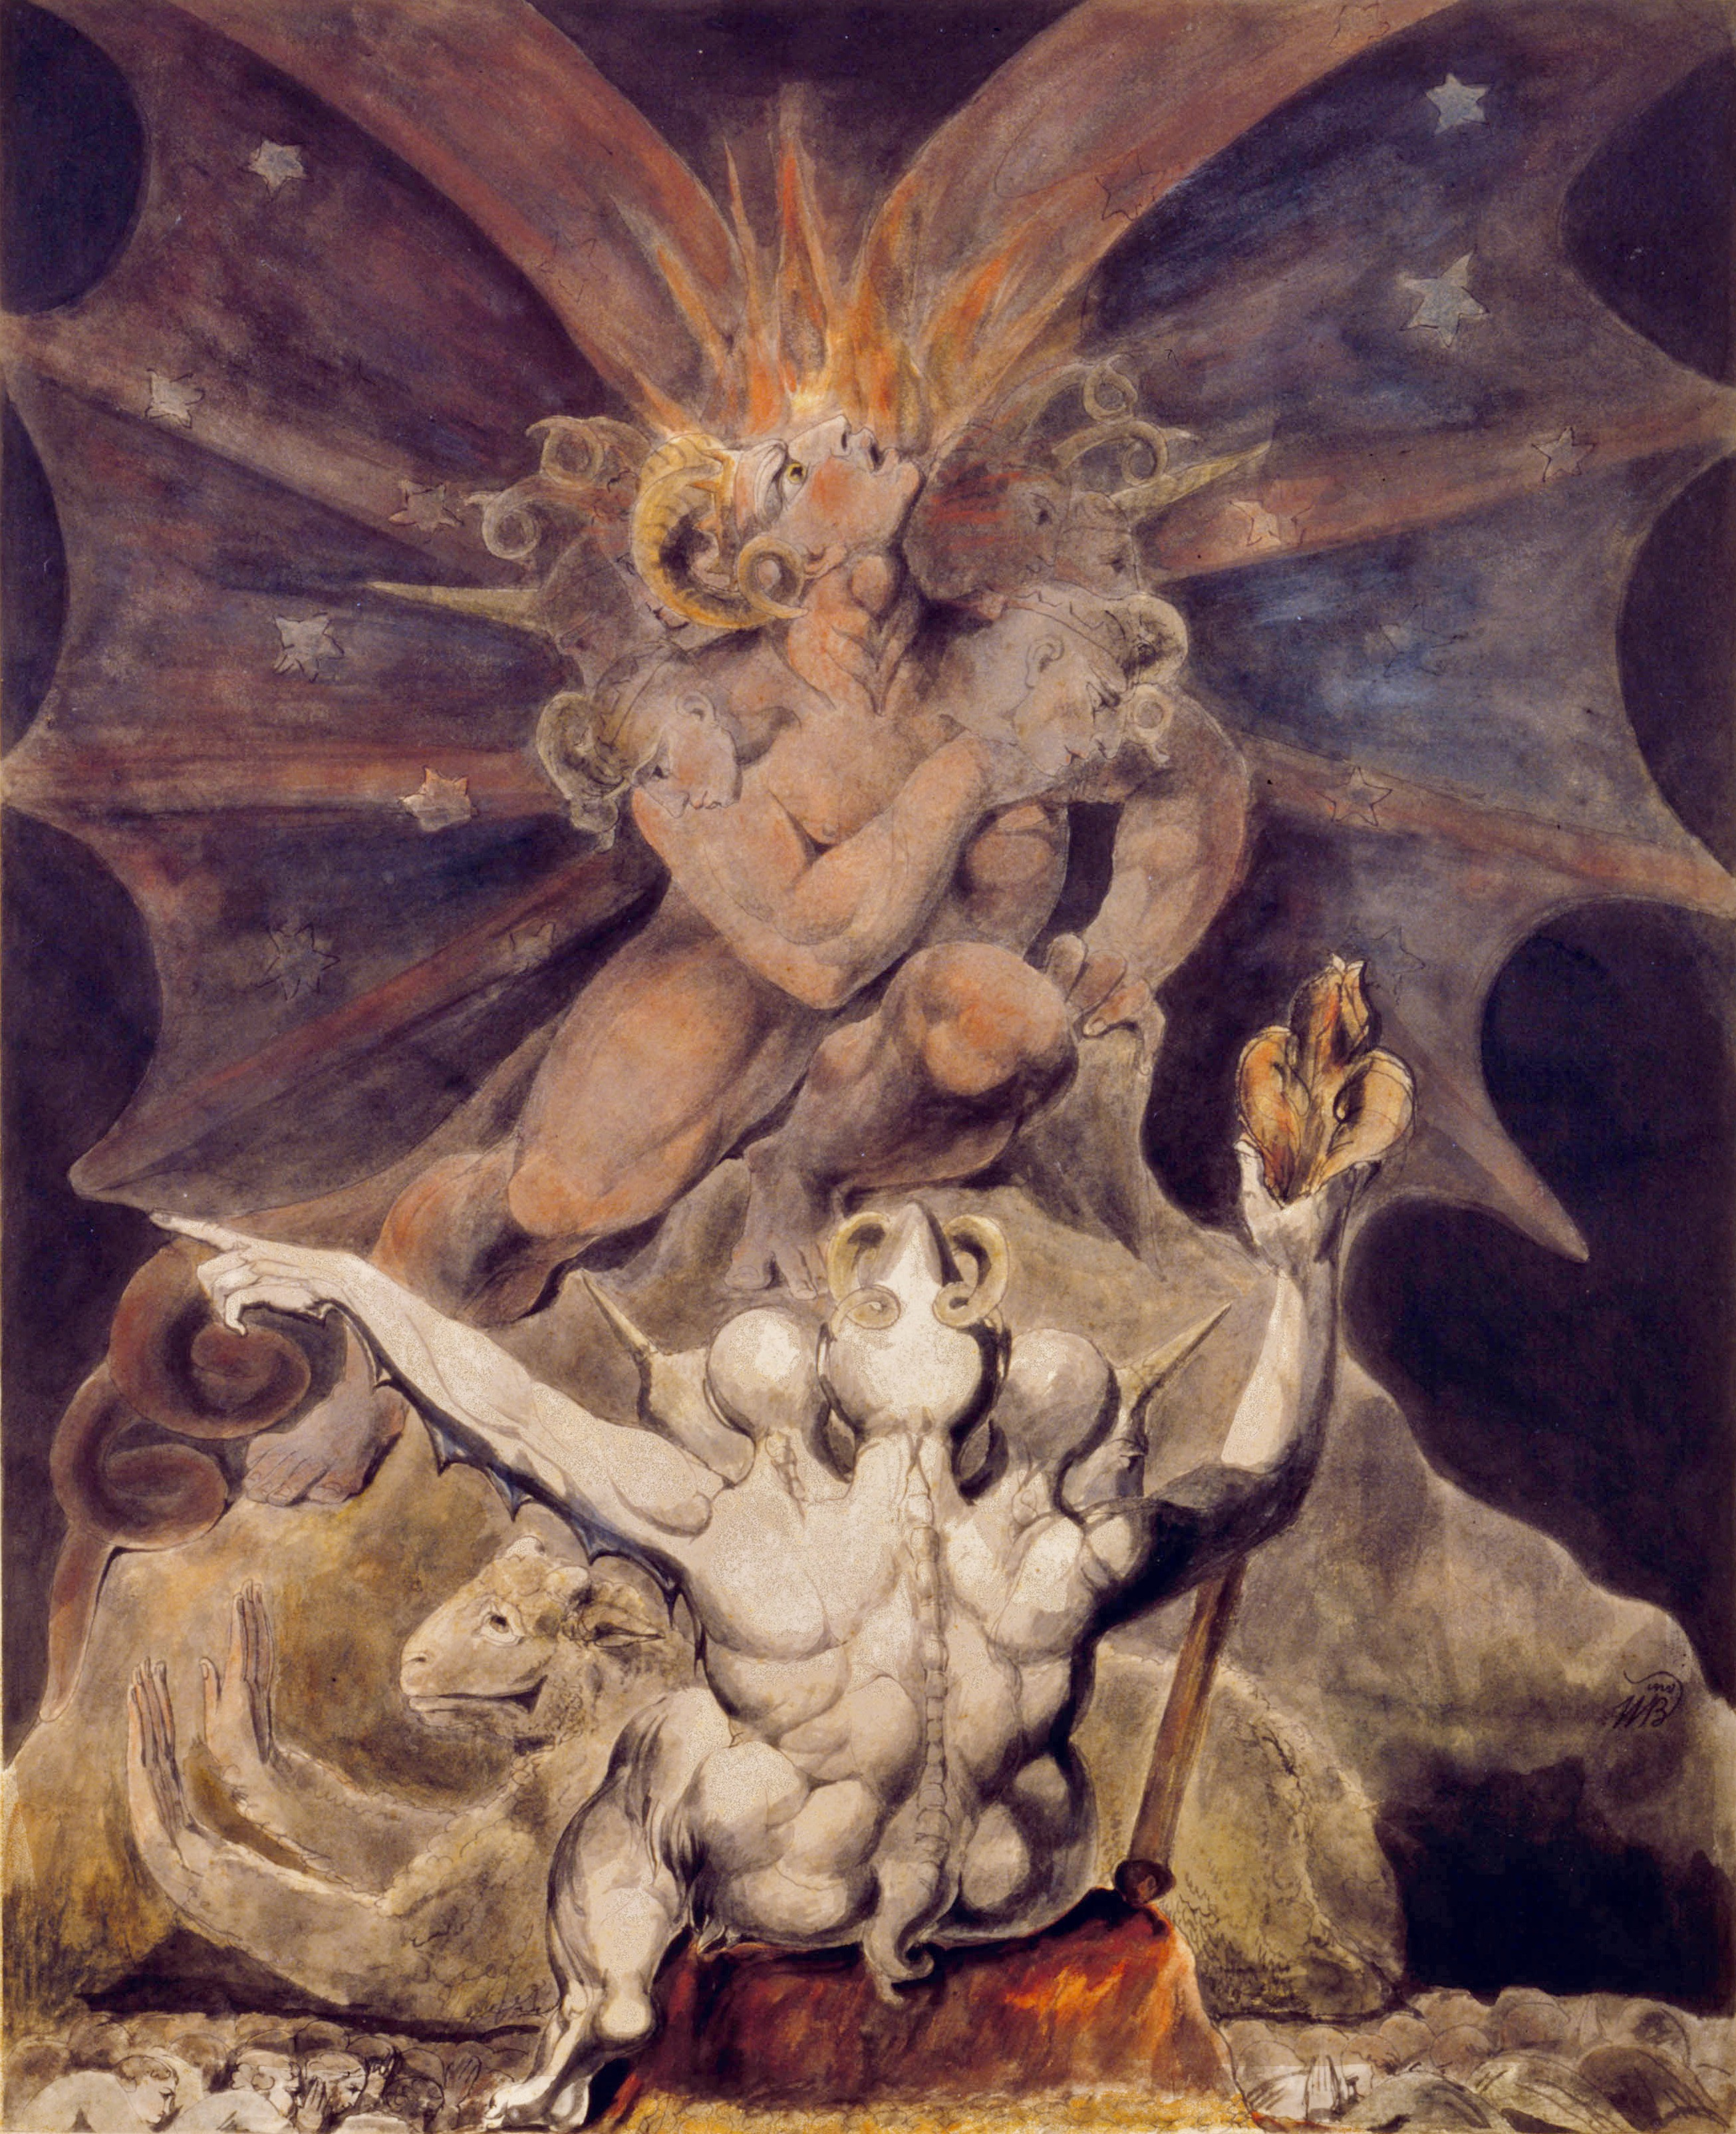
\includegraphics[width=1\textwidth]{images/illustrations/blakebeastnumber}
\end{center}